\section{The Evolution of Visual Intelligence}
\label{sec:evolution}



\paragraph{Overview: The Hierarchy of Generative Capabilities.}

As foundation models move visual generation beyond isolated image synthesis, it becomes increasingly important to articulate \emph{what capability is being improved} when we claim a model is ``more intelligent.'' Inspired by OpenAI's staged roadmap for general AI, we propose a domain-specific \textbf{5-Level Taxonomy for Visual Intelligence} that characterizes models by the \emph{type of competence} they exhibit in generation, rather than by architecture or task label.

\textbf{Why a leveled taxonomy?} The five levels reflect a \emph{nested expansion}: each subsumes its predecessors and adds one qualitatively new competence. Two operational axes separate them. \emph{How much a single forward pass can absorb}: L1 takes only a prompt; L2 adds one explicit condition; L3 absorbs rich context within one pass. \emph{Whether the system orchestrates multiple calls}: L4 introduces an external controller that orchestrates multiple passes; L5 further requires that generation be anchored in physical and causal world knowledge. Each level is made precise below and summarized in \Cref{tab:5levels}.

Progress along this taxonomy is not one-dimensional: it is a transition from \emph{passive statistical rendering} to \emph{goal-directed, physically informed visual intelligence}. This clarifies why many photorealistic systems still fail at persistent identity, long-horizon reasoning, or real-world interaction---they remain at lower capability levels. The taxonomy threads through this work: \Cref{sec:method,sec:train,sec:resource_and_infra,sec:applications} can each be read as mechanisms pushing models along this trajectory; \Cref{sec:stress_test} stress-tests each level with real-world cases; \Cref{sec:frontier} discusses what separates the current frontier from L5 simulation. See \Cref{fig:visual_intelligence_overview,tab:5levels}.

\iffalse
\begin{figure}[!htbp]
\centering
\resizebox{\textwidth}{!}{%
\begin{tikzpicture}[
    font=\sffamily,
    levelbox/.style={
        rounded corners=4pt,
        draw=black!35,
        thick,
        minimum width=4.45cm,
        minimum height=2.55cm,
        align=center
    },
    stagearrow/.style={-{Latex[length=3mm]}, thick, black!55},
    insight/.style={
        rounded corners=3pt,
        draw=black!18,
        fill=black!2,
        inner sep=4pt,
        align=center,
        font=\sffamily\footnotesize
    },
    tag/.style={
        rounded corners=2pt,
        draw=black!20,
        fill=white,
        inner sep=3pt,
        font=\sffamily\scriptsize
    }
]

\node[levelbox, fill=selfevolagent_lighter!55] (l1) at (0,0)
    {\textbf{L1: Atomic Generation}\\[-1pt]\footnotesize \textit{one-shot plausible rendering}};
\node[levelbox, fill=selfevolagent_lighter!72] (l2) at (4.9,0)
    {\textbf{L2: Conditional Generation}\\[-1pt]\footnotesize \textit{structured instruction following}};
\node[levelbox, fill=selfevolagent_light!55] (l3) at (9.8,0)
    {\textbf{L3: In-Context Generation}\\[-1pt]\footnotesize \textit{long-context, multi-ref / multi-condition}};
\node[levelbox, fill=selfevolagent_light!75] (l4) at (14.7,0)
    {\textbf{L4: Agentic Generation}\\[-1pt]\footnotesize \textit{multi-call control flow, verification, tools}};
\node[levelbox, fill=selfevolagent_dark!18] (l5) at (19.6,0)
    {\textbf{L5: World-Modeling Generation}\\[-1pt]\footnotesize \textit{causal physics and intervention effects \emph{(future)}}};

\draw[stagearrow] (l1.east) -- (l2.west);
\draw[stagearrow] (l2.east) -- (l3.west);
\draw[stagearrow] (l3.east) -- (l4.west);
\draw[stagearrow] (l4.east) -- (l5.west);

\node[font=\sffamily\bfseries\normalsize, align=center] at (9.8,2.1)
    {From passive statistical rendering to goal-directed and physically grounded visual intelligence};
\draw[-{Latex[length=3mm]}, very thick, selfevolagent_dark!85] (-2.1,1.45) -- (21.7,1.45);

\node[insight] at (2.45,-2.05) {Capability expansion:\\ \textbf{+ Controllability}};
\node[insight] at (7.35,-2.05) {Capability expansion:\\ \textbf{+ Contextual Coherence}};
\node[insight] at (12.25,-2.05) {Capability expansion:\\ \textbf{+ Closed-loop Agency}};
\node[insight] at (17.15,-2.05) {Capability expansion:\\ \textbf{+ Causal Grounding}};

\draw[stagearrow, black!40] (2.45,-1.55) -- (2.45,-0.95);
\draw[stagearrow, black!40] (7.35,-1.55) -- (7.35,-0.95);
\draw[stagearrow, black!40] (12.25,-1.55) -- (12.25,-0.95);
\draw[stagearrow, black!40] (17.15,-1.55) -- (17.15,-0.95);

\node[tag] at (0,-3.2) {OpenAI counterpart: Level 1 Chatbots};
\node[tag] at (4.9,-3.2) {Transition toward reasoning};
\node[tag] at (9.8,-3.2) {OpenAI counterpart: Level 2 Reasoners};
\node[tag] at (14.7,-3.2) {OpenAI counterpart: Level 3 Agents};
\node[tag] at (19.6,-3.2) {OpenAI counterpart: Level 4 Innovators};

\end{tikzpicture}
}
\caption{\textbf{Overview of the proposed evolution path of visual intelligence.} Progress in visual generation is not a simple increase in fidelity; it is a staged expansion from atomic generation to conditional generation, in-context generation, agentic generation, and finally world-modeling generation.}
\end{figure}
\fi

\begin{figure}[!htbp]
    \centering
    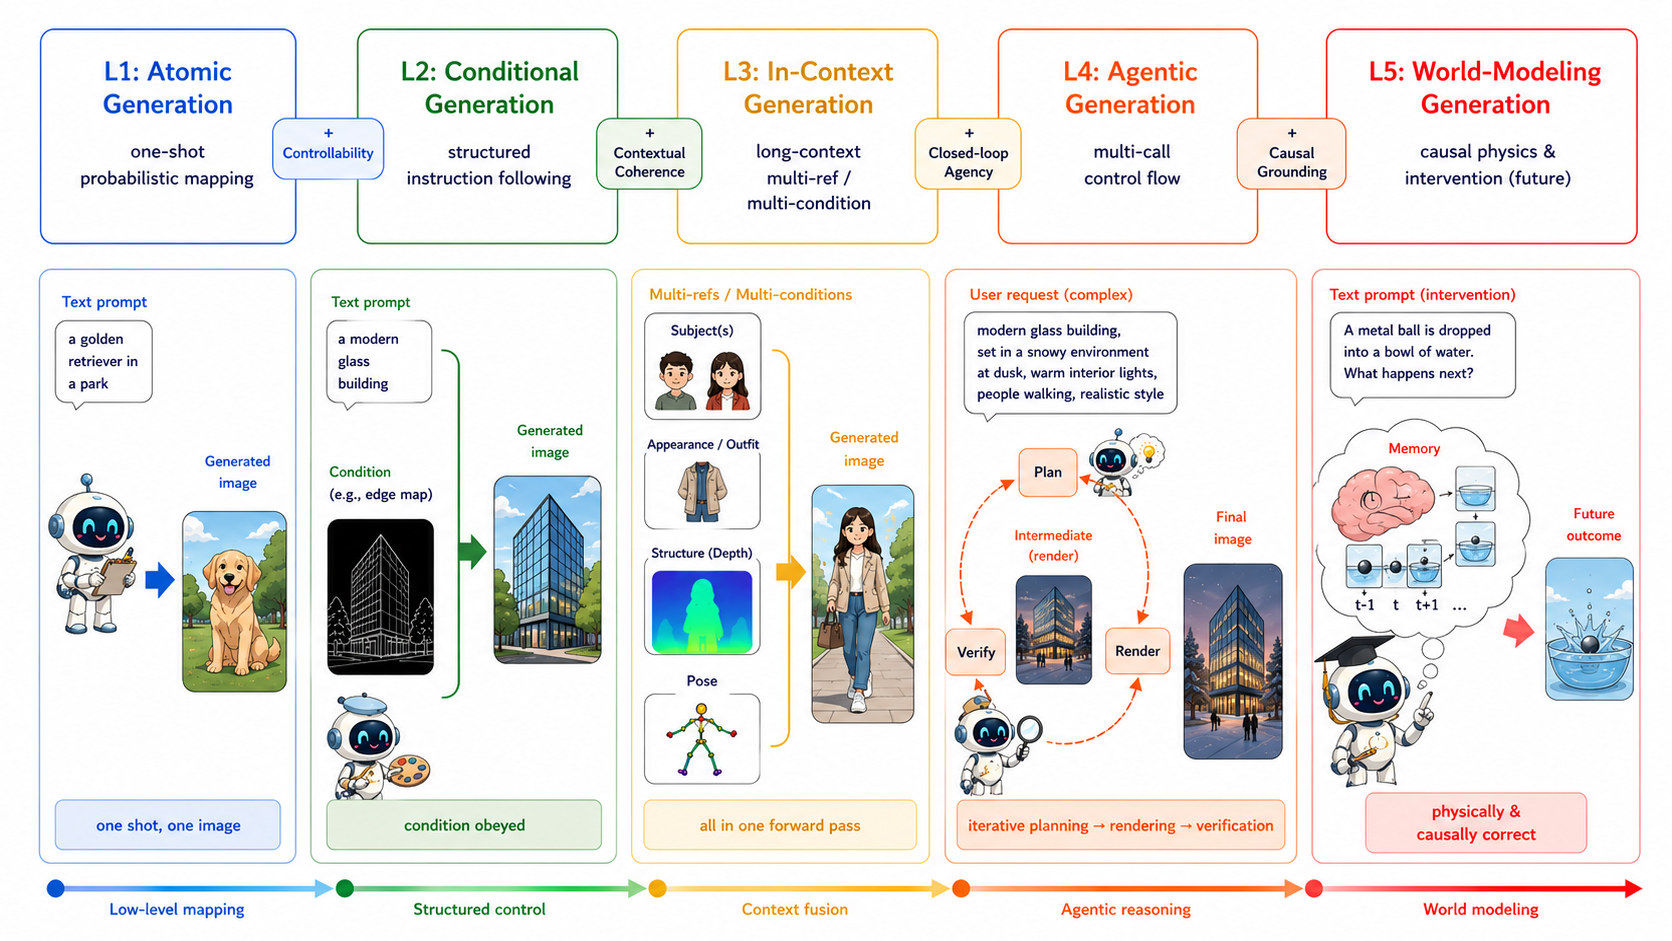
\includegraphics[width=\textwidth]{img/level/fig_5levels_overview.jpg}
    \caption{\textbf{Overview of the five-level taxonomy of visual intelligence: progression and concrete examples.} The figure unifies an abstract progression strip (top, with capability axes \textit{Controllability}, \textit{Contextual Coherence}, \textit{Closed-loop Agency}, and \textit{Causal Grounding}) with one concrete input/output example per level (bottom). \textbf{L1}: atomic text-to-image generation. \textbf{L2}: single-condition controlled generation. \textbf{L3}: multi-reference and multi-condition composition in one forward pass. \textbf{L4}: agentic generation with a planner--render--verify loop. \textbf{L5}: world-modeling generation respecting physical and domain rules. The five-level structure is a thread that runs through this survey---see \Cref{tab:5levels} for one-line definitions, the operational distinction between L3 and L4, representative methods, and key challenges.}
    \label{fig:visual_intelligence_overview}
\end{figure}



\iffalse
\begin{figure}[!htbp]
    \centering
    \fbox{\parbox[c][6cm][c]{0.95\textwidth}{\centering \textbf{[Placeholder: 5-Level concrete examples]}\\[4pt]\textit{5-panel illustration of L1--L5 with concrete input/output examples.}}}
    \caption{\textbf{Concrete examples of each level.} (DEACTIVATED placeholder; merged upward.)}
\end{figure}
\fi

\subsection{Level 1: Atomic Generation}
\label{subsec:level1}

\textbf{Definition.} Models at this level perform a direct, one-shot mapping from an input condition---typically a text prompt---to a visual output. Their role is to approximate the training distribution and produce visually convincing appearances, rather than to maintain precise structure, memory, or causal consistency. Each generation is independent.

\textbf{Representative Methods.} On the diffusion side, DDPM~\citep{ho2020denoising} introduced iterative denoising rivaling GAN samples without adversarial-training instability; Latent Diffusion Models (LDM / Stable Diffusion)~\citep{rombach2022stablediffusion} scaled it via a compressed latent space; DiT~\citep{peebles2023scalable} replaced the U-Net with a transformer that scales reliably with compute. On the autoregressive side, DALL-E~\citep{ramesh2021zero}, LlamaGen~\citep{sun2024autoregressive}, and VAR~\citep{tian2024visual} show that next-token / next-scale prediction also yields strong one-shot images. Earlier GAN systems (e.g., StackGAN~\citep{zhang2017stackgan}) established prompt-to-pixel feasibility but at limited resolution.

\textbf{Key Challenge.} The central limitation of L1 is \emph{uncontrolled variation}: the model generates what ``looks right'' according to the learned distribution, but the user has no mechanism to specify precise spatial layout, object count, identity, or structural constraints. A prompt like ``a red cube to the left of a blue sphere'' may produce a visually pleasing image where the spatial relation is violated, because the model optimizes for distributional plausibility rather than compositional correctness. We stress-test this failure mode in \Cref{sec:stress_test}, Dimension~I, where jigsaw reconstruction tasks reveal that current models default to semantic hallucination rather than geometric reasoning (\Cref{subsubsec:jigsaw_case}).


\subsection{Level 2: Conditional Generation}
\label{subsec:level2}

\textbf{Definition.} This level introduces explicit structural or multimodal constraints---such as depth maps, edge sketches, segmentation layouts, reference images, or identity embeddings---into the generative process. The model moves beyond unconstrained sampling and becomes a \emph{controllable visual constructor} that can faithfully translate prompts, controls, and references into coherent visual results. While the output now respects user-specified conditions, each generation remains a single isolated transaction: the model has no mechanism to carry forward state or memory from one generation to the next.

\textbf{Representative Methods.} ControlNet~\citep{zhang2023controlnet} injects spatial conditions (edges, depth, pose) into a frozen diffusion backbone via a trainable copy. IP-Adapter~\citep{ye2023ip} and InstantID~\citep{wang2024instantid} inject reference-image features through cross-attention for identity control; DreamBooth~\citep{ruiz2023dreambooth} and Textual Inversion~\citep{gal2022image} extend the model's concept vocabulary from a few reference images. Layout-to-image methods like GLIGEN~\citep{li2023gligen} and CreatiLayout~\citep{CreatiLayout} take bounding boxes or region semantics as input. On the architecture side, SD3~\citep{esser2024stablediffusion3} builds L2 conditioning into the backbone via MM-DiT. The shared property: the output is a \emph{constrained} sample satisfying user-specified conditions, not a free sample.

\textbf{Key Challenge.} The central challenge at L2 is \emph{spatial precision and attribute binding}: ensuring that the model places the right content in the right region with the right attributes, rather than merely producing an image globally consistent with the prompt. Even with explicit layout constraints (e.g., ``left box: red hat; right box: blue scarf''), current models frequently exhibit attribute leakage (the scarf inherits the hat's color) or spatial confusion (left-right reversal). We examine these failure modes in detail in \Cref{sec:stress_test}, Dimension~I.


\subsection{Level 3: In-Context Generation}
\label{subsec:level3}

\textbf{Definition.} L3 is still a \emph{single forward pass}, but one that absorbs \emph{rich context}: multiple references, multiple conditions, or an accumulated history of prior generations and edits. The model has no external controller---memory is implicit in the input. This framing reveals why multi-turn editing belongs at L3, not at L4: each round is a single forward pass over a growing input sequence (image$_0$, edit$_1$, image$_1$, edit$_2$, $\dots$), with the model producing image$_k$ in one shot. The challenge is analogous to the difference between answering a single question (L2) and sustaining a coherent multi-turn conversation where earlier statements constrain later ones---still one model, one forward pass, just with more context.

\textbf{Representative Methods.} L3 capability appears in three forms, all sharing the operational signature: one forward pass over rich input. \textit{(i)~Multi-reference / multi-condition composition.} The model fuses several references (subject, outfit, scene) and structural conditions (depth, pose) into one coherent output---the regime that recent unified backbones target most directly. \textit{(ii)~Multi-turn editing with cumulative context.} SEED-Data-Edit~\citep{ge2024seed} and ImgEdit~\citep{ye2025imgedit} let users chain successive edits (``change background,'' then ``add sunglasses,'' then ``shorten hair''); each turn is one forward pass over the accumulated history, requiring pixel-level fidelity in unedited regions---a property favoring VAE-based representations over purely semantic encoders. Cross-panel storytelling extends this: StoryMaker~\citep{zhou2024storymaker} and Visual Persona~\citep{nam2025visual} keep character identity stable across panels via multi-pose supervision and full-body identity representations. \textit{(iii)~Reasoning trace inside one pass.} ReasonGen-R1~\citep{zhang2025reasongen} and T2I-R1~\citep{jiang2025t2i} interleave a textual reasoning trace with image generation inside a single AR sequence---still one forward pass, with no external controller deciding when to stop, placing them at L3.

\textbf{Key Challenge.} The defining difficulty at L3 is \emph{coherence preservation under cumulative context}: the model must update what the user asks (expression, pose, background) while keeping everything else pixel-faithful as the input context grows. Errors accumulate---a small identity drift in one editing step compounds across subsequent steps, and even VAE reconstruction error becomes visible after several round-trips. We examine these failure modes in \Cref{sec:stress_test}, Dimension~IV, and the specific case of cross-frame identity preservation in \Cref{subsubsec:video_re-rendering_case}.

\textbf{Method vs.\ probe.} The L3 classification above is about \emph{method}: a naive multi-turn system stays at L3 because each round is one forward pass with no controller deciding what to verify or roll back. The same task surface, however, is the cleanest \emph{probe} for L4 \emph{capability}: a system that detects mid-sequence identity drift and silently restores, or triggers re-rendering on context conflict, exhibits L4 even though mechanically each round is still one forward pass. \Cref{sec:stress_test}, Dimension~IV uses this dual nature as its probe design.

\iffalse
\begin{highlightbox}{Key Insight: Why Multi-Turn Editing Lives at L3, Not L4}

Multi-turn editing \emph{looks} like an iterative agent loop, but mechanically it is just a single-forward-pass system whose context grows each round. The model sees the accumulated \emph{(image$_0$, edit$_1$, image$_1$, edit$_2$, \dots)} sequence as input and produces image$_k$ in one forward pass; memory is implicit in the input, not in any controller. Concretely, Wan-Image's bidirectional attention across an image series, Hunyuan~3.0's TI2TI chain-of-thought, and the inferred Nano-Banana multi-round protocol all fit this pattern. By the operational test of one forward pass over rich context vs.\ multiple passes stitched by a controller (\Cref{tab:5levels}), they remain L3---per-call capacity stretched by long context---rather than L4, which requires an \emph{external control flow} that decides what to call, when to verify, and when to stop. Reasoning-augmented generation (T2I-R1, ReasonGen-R1) lands in the same place: a CoT trace inside one AR sequence is still one forward pass, otherwise every CoT-LLM would qualify as an agent. Treating multi-turn as L4 conflates richer context with genuine orchestration and obscures the actual research frontier between the two regimes.
\end{highlightbox}
\fi


\subsection{Level 4: Agentic Generation}
\label{subsec:level4}



\textbf{Definition.} At L4, generation becomes one action inside a control loop rather than the final output. Following the LLM literature \citep{anthropic2024agents}, we use \emph{agentic} in the strong sense: a system qualifies as L4 when it (i)~\textbf{dynamically decides} the next action based on observations rather than following a pre-scheduled pipeline, (ii)~operates inside an \textbf{environment feedback loop} where outputs change state and the new state shapes subsequent inputs, (iii)~\textbf{persists toward a long-horizon goal} across multiple forward passes, and (iv)~\textbf{decides when to terminate}. The L3-vs-L4 boundary is therefore about \emph{autonomy over the trajectory}, not the number of user turns.

\textbf{Representative Methods.} Following Anthropic's distinction between \emph{workflows} (LLMs and tools orchestrated through pre-defined code paths) and \emph{agents} (LLMs that dynamically direct their own processes and tool use) \citep{anthropic2024agents}, current L4-related systems span a spectrum.

\textit{Workflow side.} GEMS~\citep{he2026gems} composes a fixed planner$\to$decomposer$\to$verifier$\to$refiner loop with trajectory-level memory; Gen-Searcher~\citep{feng2026gen} extends it with web search and evidence collection. Verification and retrieval become first-class building blocks, but the control flow is engineered, not chosen by the model.

\textit{Agent side.} JarvisArt~\citep{lin2025jarvisart} dynamically selects from 200+ Lightroom tools based on user intent and intermediate state. CoT-VLA~\citep{zhao2025cotvla} and UniPi~\citep{du2023unipi} are the embodied analog: the model predicts visual states conditioned on actions and uses these predictions to choose subsequent actions in a robotic policy loop.

Most current visual L4 systems sit on the workflow end; full agentic systems---where the model chooses its own actions toward a long-horizon goal in a single closed loop---remain rare. Two boundary clarifications: (a)~unified multimodal backbones (Transfusion~\citep{zhou2024transfusion}, BAGEL~\citep{deng2025bagelemerging}, OmniMamba~\citep{zou2025omnimamba}) are \emph{not} L4 agents themselves but provide the shared state space on top of which planning and tool use become easier; (b)~boundary with L5: at L4, generation is a \emph{means} in a policy loop (CoT-VLA predicts visual states for downstream control); at L5, generation itself must encode causal world dynamics.

\textbf{Key Challenge.} The defining challenge at L4 is \emph{grounded verification under intervention}: the system must verify not only the final image but each intermediate \emph{decision}---what to search, what tool to invoke, when to stop---against whether it is the right next action for the current state. The harder a system pushes from workflow- toward agent-side, the more its trajectory depends on its own decision quality. Memory and retrieval (GEMS, Gen-Searcher) extend competence yet expose new failure modes: noisy evidence, brittle verifier signals, trajectories optimizing proxies rather than the goal. Tool-grounded settings (JarvisArt) demand correct executable edits with content preservation and local precision, not just plausible pixels. L4 systems fail not because they cannot render, but because they cannot yet \emph{reliably decide, verify, and correct} inside an open-ended loop. \Cref{sec:stress_test} Dimensions~III and IV surface this through fragile reasoning traces and silent drift in multi-turn editing.



\begin{table}[!htp]
\centering
\caption{\textbf{Comparative taxonomy of visual intelligence.} Our five-level framework organizes progress in visual generation as a nested expansion of capability, drawing parallels to OpenAI's general AI roadmap. Each level subsumes its predecessors while introducing a qualitatively new competence, a distinct set of representative methods, and a defining challenge that separates statistical plausibility from genuine visual intelligence. The \textit{One-Line Definition} column captures the operational signature of each level---most importantly, that L3 remains a single forward pass over rich context, while L4 is the regime where multiple forward passes are stitched by an external control flow.}
\label{tab:5levels}
\resizebox{\textwidth}{!}{%
    \begin{tabular}{@{}c l l l l l l@{}}
        \toprule[1pt]
        \textbf{Level} & \textbf{Visual Paradigm} & \textbf{One-Line Definition} & \textbf{Core Characteristic} & \textbf{Representative Methods} & \textbf{Key Challenge} & \textbf{AI Counterpart} \\ \midrule
        \textbf{L1} & \textbf{Atomic Generation} & \makecell[l]{One forward pass without \\ explicit constraints; sample a \\ plausible image from text alone} & \makecell[l]{Stochastic Plausibility \\ (Distribution Matching)} & \makecell[l]{DDPM, DiT, LDM/SD, \\ LlamaGen, VAR} & \makecell[l]{Uncontrolled variation; \\ no spatial precision} & \makecell[l]{OpenAI L1 \\ (Chatbots)} \\ \midrule
        \textbf{L2} & \textbf{Conditional Generation} & \makecell[l]{One forward pass with a \\ single explicit condition \\ (structure / reference / \\ source-image $+$ instruction)} & \makecell[l]{Compositional \\ Controllability} & \makecell[l]{ControlNet, IP-Adapter, \\ GLIGEN, SD3} & \makecell[l]{Attribute binding \& \\ spatial precision} & \makecell[l]{Transition toward \\ Reasoning} \\ \midrule
        \textbf{L3} & \textbf{In-Context Generation} & \makecell[l]{One forward pass over rich \\ context: multi-reference, \\ multi-condition, accumulated \\ history, or multi-output} & \makecell[l]{Contextual Coherence \\ (Visual Logic \& Memory)} & \makecell[l]{SEED-Data-Edit, ImgEdit, \\ StoryMaker, Visual Persona} & \makecell[l]{Identity preservation \\ under state change} & \makecell[l]{OpenAI L2 \\ (Reasoners)} \\ \midrule
        \textbf{L4} & \textbf{Agentic Generation} & \makecell[l]{Multiple forward passes \\ with control flow: plan, \\ verify, invoke tools, refine} & \makecell[l]{Closed-loop Agency \\ (Perception-Action-Feedback)} & \makecell[l]{GEMS, Gen-Searcher, \\ JarvisArt, CoT-VLA} & \makecell[l]{Grounded verification \\ \& self-correction} & \makecell[l]{OpenAI L3 \\ (Agents)} \\ \midrule
        \textbf{L5} & \makecell[l]{\textbf{World-Modeling} \\ \textbf{Generation} \textit{(future)}} & \makecell[l]{Generation anchored by an \\ internalized world model; \\ discriminative tasks and \\ domain-structured generation \\ emerge as consequences} & \makecell[l]{Causal Simulation \\ (Physics \& Intervention)} & \makecell[l]{Genie 2, GameNGen, \\ Oasis, UniSim, GAIA-1} & \makecell[l]{Causal faithfulness; \\ physical plausibility} & \makecell[l]{OpenAI L4 \\ (Innovators)} \\
        \bottomrule[1pt]
    \end{tabular}%
    }
\end{table}



\subsection{Level 5: World-Modeling Generation \textit{(future)}}
\label{subsec:level5}

\textbf{Definition.} L5 is reached when a model internalizes stable representations of dynamics, physics, and intervention effects---a \emph{world simulator}, not just an appearance generator. Where L4 agents reason from learned correlations, L5 demands prediction of what \emph{would actually happen} under a specific action in a specific physical context. The most fully realized L5 demonstrations today appear in interactive video and embodied settings; we treat them as case studies of L5 \emph{capability}, not as methodological focus.

\textbf{Representative Methods.} \emph{Neural game engines} provide the most vivid demonstrations: Genie~2~\citep{parker2024genie2} generates 3D environments learned from passive video, with persistent object behavior; GameNGen~\citep{valevski2024gamenngen} replaces DOOM's hand-coded engine with a diffusion model rendering frames conditioned on player actions at interactive frame rates; Oasis~\citep{oasis2024} scales this to Minecraft. In embodied settings, UniSim~\citep{yang2024unisim} is a universal visual simulator for manipulation and navigation; GAIA-1~\citep{hu2024gaia1} generates controllable driving scenarios conditioned on vehicle actions. Image-side, L5 also encompasses \emph{world-knowledge grounding}: rendering scenarios that respect gravity, fluid dynamics, material properties, or domain rules---probed by benchmarks like PhyBench~\citep{meng2024phybench} and WISE~\citep{niu2025wise}.

\textbf{Key Challenge.} The decisive challenge is \emph{causal faithfulness}: whether the generated future state reflects the causal consequences of an intervention, not merely its statistical correlates. A photorealistic rollout that ignores the commanded steering or misrepresents contact dynamics is worse than useless for downstream policy learning---it corrupts the training signal. Current models learn correlations without internalizing physical laws and fail under unusual mechanisms or extreme maneuvers. Evaluation itself is a fundamental barrier at L5: judging whether a scene is \emph{physically correct} and \emph{causally consistent} requires benchmarks beyond perceptual quality---verifying how a scene \emph{works}, not what it \emph{looks like}. We examine this gap through fluid-dynamics counterfactuals (\Cref{subsubsec:fluid_dynamics_case}), action-conditioned driving (\Cref{subsubsec:driving_collision_case}), robotic manipulation (\Cref{subsubsec:robot_grasp_case}), and trajectory synthesis (\Cref{subsubsec:trajectory_synthesis}).



